Cette partie montrera l’ensemble des maquettes de la future interface du logiciel.

\subsection{Fenêtre principale}

\begin{figure}[H]
  \centering
  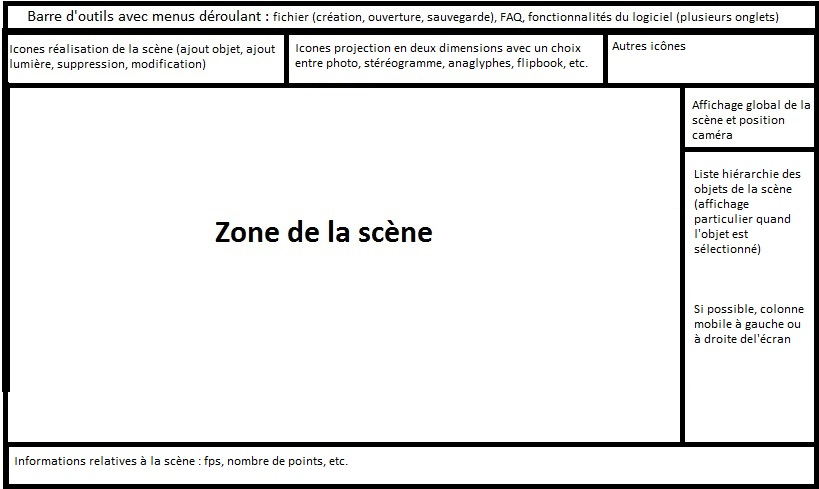
\includegraphics[scale=0.6]{fenetreprincipale}
  \caption{Fenêtre principale}
  \label{fig:fenppale}
\end{figure}

La fenêtre principale \ref{fig:fenppale} se détaille comme suit :

\begin{itemize}
\item Barre d'outils avec menus déroulants
  
  Ce bandeau supérieur correspond à un bandeau supérieur de logiciel classique, comme on le trouve par exemple dans le logiciel Meshlab.

  L’intérêt de ces menus déroulants est de proposer l’accès à l’ensemble des fonctionnalités du logiciel. Parmi ces menus se trouvent quelques redondances avec des icônes présentes dans d’autres parties de la fenêtre principale, afin que l’utilisateur puisse choisir l’utilisation du logiciel qui lui convient le mieux.
  
\item Icônes de réalisation de la scène
  
  Les icônes permettant de réaliser la gestion des objets et des lumières de la scène : il sera possible d’ajouter un objet ou de le modifier à partir de ces icônes.

\item Icônes de projection en deux dimensions
  
  L’ensemble des icônes permettant d’obtenir l’un des rendus possibles à l’aide du logiciel, c’est-à-dire quatre icônes pour : une projection en deux dimensions classique, la création d’un anaglyphe, la création d’un stéréogramme et la création d’un flipbook.
  
  L’ensemble de ces icônes permettra d’ouvrir une nouvelle fenêtre et de choisir les paramètres de l’image à obtenir.

\item Autres icônes
  
  Cette zone pourra contenir d’autres icônes, qui seront triées et rassemblées en fonction de leurs cas d’utilisation.

\item Zone de la scène
  
  Vu de la scène du point de vue de la caméra. L’utilisateur pour s’y déplacer librement via la caméra pour pouvoir l’observer depuis différents angles. Il pourra également sélectionner des objets pour les déplacer, modifier leur orientation, les redimensionner ou les supprimer.

\item Liste des objets de la scène
  
  L’ensemble des objets présents dans la scène listés : l’utilisateur pourra cliquer sur le nom d’un objet afin de le sélectionner et de pouvoir agir dessus.

\item Informations relatives à la scène
  
  Des informations intéressantes pour l’utilisateur par rapport à la scène et à son affichage seront affichées : le nombre d’objets dans la scène, le nombre de points, ou encore la qualité d’affichage en frames par seconde. Cette zone pourra également servir à l’affichage de messages informatifs ou de messages d’erreurs à l’intention de l’utilisateur.
\end{itemize}

\subsection{Fenêtre de chargement d'un objet}

\begin{figure}[h]
  \centering
  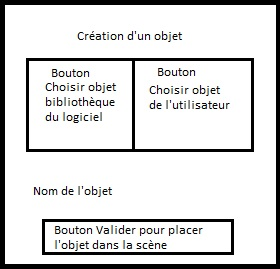
\includegraphics{chargement}
  \label{fig:chargement}
  \caption{Fenêtre de chargement d'un objet}
\end{figure}

\paragraph{}
L'image \ref{fig:chargement} schématise la fenêtre de chargement d’un nouvel objet. L’utilisateur du logiciel doit d’ores et déjà avoir ouvert une scène. Il pourra ensuite choisir d’y insérer un nouvel objet grâce à la fenêtre ci-dessus, en choisissant un modèle à ouvrir ainsi que le nom de l’objet dans la scène.

\paragraph{}
Pour le choix du modèle 3D, l’utilisateur pourra utiliser soit la bibliothèque du logiciel soit ses propres fichiers. Toutefois, seules les extensions OBJ et PLY seront acceptées.

\paragraph{}
Une fois toutes les informations entrées, l’utilisateur pourra cliquer sur le bouton Valider pour passer en mode Modification de l’objet et placer son objet dans sa scène.

\newpage

\subsection{Interface de modification d'un objet}


\begin{figure}[h]
  \centering
  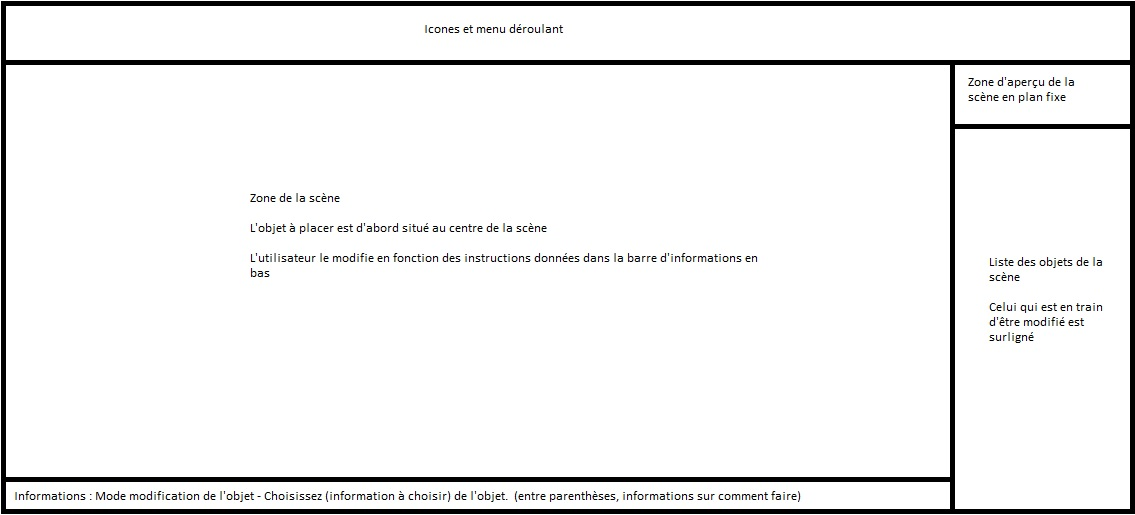
\includegraphics[scale=0.5]{interfacemodifs}
  \label{fig:interfacemodifs}
  \caption{Interface de modification d'un objet}
\end{figure}

\paragraph{}
Une fois qu’il aura choisi le modèle à placer, l’utilisateur verra de nouveau la fenêtre principale s’afficher, et devra suivre les informations indiquées dans la barre Informations en bas de la fenêtre pour modifier la position, l’orientation et la taille de l’objet.

\paragraph{}
S’il souhaite de nouveau effectuer des modifications sur son objet, il devra repasser en mode Modification de l’objet, et retrouvera la même interface \ref{fig:interfacemodifs}. Il devra à chaque fois obligatoirement passer par les trois modes de modification : position, orientation, taille.

\subsection{Fenêtre de choix des options du rendu}

\begin{figure}[h]
  \centering
  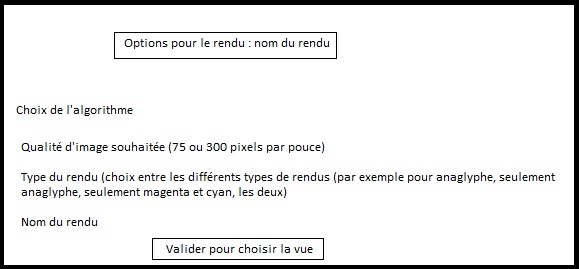
\includegraphics[scale=0.6]{choixoptionsrendu}
  \label{fig:optionsrendu}
  \caption{Choix des options du rendu}
\end{figure}

\paragraph{}
La fenêtre \ref{fig:optionsrendu} s’ouvre lorsque l’utilisateur clique sur le bouton de création d’une projection, d’un anaglyphe, d’un autostéréogramme ou d’un flipbook. Il devra alors choisir l’algorithme à utiliser pour le rendu souhaité (un ou plusieurs algorithmes pourront être proposés), la qualité d’image qu’il souhaite obtenir, ainsi que les types de retour qu’il souhaite obtenir si plusieurs choix existent. Par exemple, dans le cas d’un anaglyphe, le retour pourra contenir ou bien uniquement l’anaglyphe, ou bien les deux vues rouge et cyan, ou bien les deux.

\paragraph{}
L’utilisateur choisira ensuite le nom du rendu et appuiera sur le bouton ``Valider'' pour passer en mode de sélection de la vue. Ce mode reviendra sur la fenêtre principale du logiciel, et des informations seront données à l’utilisateur pour sélectionner la vue qu’il souhaite.

\paragraph{}
Toutes les informations seront obligatoirement complétées pour pouvoir accéder au mode de sélection de la vue.

\subsection{Fenêtre d'affichage du rendu}

\begin{figure}[H]
  \centering
  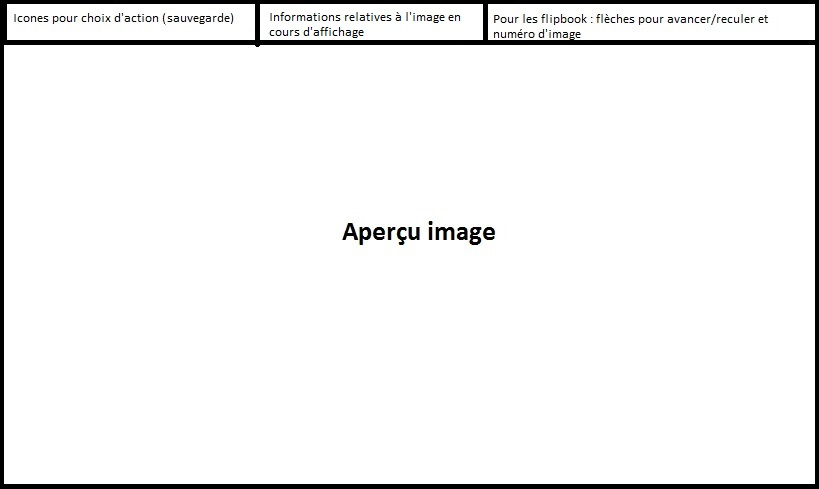
\includegraphics[scale=0.6]{apercuimage}
  \label{fig:apercu}
  \caption{Affichage du rendu}
\end{figure}

Une fois l'action paramétrée, le rendu s'affiche dans la fenêtre \ref{fig:apercu} dont les options sont détaillés ci-dessous.

\begin{itemize}

\item Zone de choix d’action
  
  Cette zone contiendra des icônes pour indiquer à l’utilisateur les choix qui s’offrent à lui. On trouvera par exemple une icône pour l’enregistrement du rendu, qui ouvrira une nouvelle fenêtre pour laisser le choix à l’utilisateur de ce qu’il souhaite enregistrer.
  
\item Zone d’affichage des informations
  
  Cette zone concernera uniquement l’image en cours d’affichage dans la zone d’aperçu. On détaillera ici la taille de l’image et sa qualité en pixels par pouce.
  
\item Zone de défilement
  
  Cette zone contiendra des flèches de déroulement vers la gauche ou vers la droite pour permettre à l’utilisateur de voir l’ensemble des images obtenues, ainsi qu’un ou plusieurs boutons pour pouvoir afficher un GIF ou le stopper.
  
\item Zone d’aperçu de l’image
  
  S’affichera ici l’image obtenue après la requête d’un utilisateur.
  
\end{itemize}
